\chapter{Perkembangbiakan Aseksual dan Pengklonaan pada Tumbuhan}\label{ch:b2:asexual-reproduction}

Di sebuah lembah di Utah berdiri sebuah hutan berisi empat puluh tujuh
ribu batang aspen yang merupakan satu tumbuhan: tiap batangnya tumbuh
dari sistem akar yang sama, tiap selnya mengusung genom yang sama, dan
individunya berumur sekitar empat belas ribu tahun serta berbobot enam
ribu ton. Tiap arbei di dalam satu keranjang pasar swalayan yang
sevarietas adalah sekeping satu tumbuhan yang dilipatgandakan lewat
sulur; tiap pisang Cavendish di Bumi adalah setek dari setek satu
tumbuhan. Tumbuhan, tidak seperti sebagian besar hewan, dapat membuat
individu baru tanpa seks --- dari sebuah batang, sebuah akar, sehelai
daun, satu sel di dalam labu. Bab ini menelaah bagaimana mereka
melakukannya, bagaimana pekebun memanfaatkannya, dan apa yang harus
dibayar sebuah garis keturunan untuk melepaskan \omterm{def:b2:meiosis-heredity:meiosis}{meiosis} serta
pembuahan: yaitu pertanyaan mengapa seks ada sama sekali.

\section{Pelipatgandaan vegetatif}

\begin{definition}[Klon, genet, ramet]\label{def:b2:asexual-reproduction:clone}
\index{klon}\index{genet}\index{ramet}\index{pelipatgandaan vegetatif}
\emph{Perkembangbiakan aseksual} menghasilkan individu baru dari satu
tetua lewat mitosis semata, tanpa \omterm{def:b2:meiosis-heredity:meiosis}{meiosis} maupun pembuahan:
keturunannya adalah sebuah \emph{klon}, serupa secara genetik dengan
tetuanya dan dengan sesamanya, kecuali \omterm{def:b2:genome-diversification:mutation}{mutasi} soma yang menimbun. Pada
tumbuhan bentuk yang lazim adalah \emph{pelipatgandaan vegetatif}, yang
di dalamnya sebagian tubuhnya --- batang, akar, daun --- berakar lalu
menjadi tumbuhan tersendiri. Sebuah \emph{genet} adalah individu
genetiknya, segala sesuatu yang tumbuh dari satu zigot; sebuah
\emph{ramet} adalah satu satuannya yang terpisah secara fisiologi.
Sebidang arbei dapat memuat seribu ramet satu genet; hutan aspennya
adalah satu genet. Pelipatgandaan vegetatif mungkin terjadi karena sel
tumbuhan mempertahankan kesanggupan membelah dan membentuk organ apa
pun --- mereka \emph{totipoten} --- dan karena tumbuhan tumbuh dari
meristem yang dapat dibangunkan kembali nyaris di mana pun.
\end{definition}

\begin{proposition}[Organ pelipatgandaan vegetatif]\label{prop:b2:asexual-reproduction:organs}
\index{sulur}\index{rimpang}\index{umbi batang}\index{umbi lapis}
Tumbuhan telah mengembangkan muslihat yang sama dari tiap organnya.
Dari batang: \emph{sulur} atau \emph{stolon}, yaitu pucuk mendatar
sepanjang tanah yang berakar pada buku-bukunya (arbei, ranunkulus
menjalar); \emph{rimpang}, yaitu \omterm{prop:b2:asexual-reproduction:horticulture}{batang bawah} tanah mendatar yang
bercabang dan terpecah (rumput teki, iris, jahe, paku kawat);
\emph{\omterm{prop:b2:asexual-reproduction:organs}{umbi batang}}, yaitu ujung rimpang yang menggembung dan menyimpan
pati serta mengusung tunas, yakni ``matanya'' (kentang); \emph{bonggol},
yaitu pangkal batang tegak yang menggembung (krokus); \emph{umbi
kecil}, yaitu \omterm{prop:b2:asexual-reproduction:organs}{umbi lapis} kecil yang terbentuk pada ketiak daun atau
pada kepala \omterm{def:b2:angiosperm-reproduction:flower}{bunganya} (bawang putih, sebagian bawang). Dari daun:
\emph{\omterm{prop:b2:asexual-reproduction:organs}{umbi lapis}}, yaitu tunas yang terbungkus daun simpanan yang
berdaging lalu terbelah menjadi umbi anak (bawang bombai, tulip);
tumbuhan kecil di sepanjang tepi daunnya, lengkap dengan akar, yang
rontok (\emph{Kalanchoe}). Dari akar: \emph{tunas akar}, yaitu pucuk
yang menjulang dari akar mendatar (aspen, prem liar, frambus). Lewat
\emph{pemecahan}: sekeping ranting dedalu yang hanyut lalu berakar,
sehelai ental mata lele yang terbelah. Dalam tiap kasusnya sebuah organ
simpanan atau sebuah meristem dibawa sejarak pendek, dan anaknya memulai
hidup dengan pasokan makanan yang tak tertandingi \omterm{def:b2:angiosperm-reproduction:seed}{biji} mana pun.
\end{proposition}

\begin{omfigure}
\begin{tikzpicture}[every node/.style={font=\scriptsize}]
  % runner
  \begin{scope}
    \draw[thick] (0,0) -- (3.6,0);
    \foreach \x in {0,1.8} { \draw[thick, omExo!70!black, fill=omExo!30] (\x,0) .. controls (\x-0.3,0.6) and (\x+0.3,0.6) .. (\x,0); \foreach \a in {60,90,120} \draw[thick, omExo!70!black] (\x,0) -- ++(\a:0.7); \draw[gray] (\x,0) -- ++(-100:0.4) (\x,0) -- ++(-70:0.4); }
    \draw[thick, omThm] (0.2,0.15) .. controls (0.9,0.55) and (1.2,0.55) .. (1.8,0.1);
    \draw[thick, omThm] (2.0,0.15) .. controls (2.7,0.55) and (3.0,0.55) .. (3.5,0.1);
    \draw[thick, omExo!70!black] (3.5,0.1) -- ++(80:0.4); \draw[gray] (3.5,0.1) -- ++(-80:0.3);
    \node[below, align=center] at (1.8,-0.55) {sulur (arbei):\\pucuk mendatar yang berakar pada bukunya};
  \end{scope}
  % rhizome and tuber
  \begin{scope}[xshift=5.2cm]
    \draw[gray, dashed] (-0.2,0) -- (3.8,0);
    \draw[very thick, omProp!80!black] (0,-0.5) -- (3.4,-0.5);
    \foreach \x in {0.6,2.0} \draw[thick, omExo!70!black] (\x,-0.5) -- (\x,0.7) (\x,0.3) -- ++(40:0.4) (\x,0.3) -- ++(140:0.4);
    \draw[thick, omProp!80!black, fill=omProp!40] (3.4,-0.5) ellipse (0.45 and 0.3);
    \foreach \p in {(3.2,-0.3),(3.6,-0.35),(3.7,-0.6)} \fill[omThm] \p circle (0.04);
    \foreach \x in {0.3,1.3,2.5} \draw[gray] (\x,-0.5) -- (\x,-0.9);
    \node[below, align=center] at (1.8,-1.05) {rimpang dan umbi batang (kentang):\\batang bawah tanah,\\tunas (mata) pada umbinya};
  \end{scope}
  % bulb
  \begin{scope}[xshift=12.2cm]
    \draw[thick, fill=omExo!15] (0,-0.9) .. controls (-0.9,-0.6) and (-0.9,0.9) .. (0,1.0) .. controls (0.9,0.9) and (0.9,-0.6) .. (0,-0.9);
    \foreach \r in {0.55,0.35} \draw[thick] (0,-0.75) .. controls (-\r,-0.5) and (-\r,0.6) .. (0,0.8) .. controls (\r,0.6) and (\r,-0.5) .. (0,-0.75);
    \fill[omExo!60!black] (-0.1,-0.75) rectangle (0.1,0.3);
    \draw[thick, omThm, fill=omThm!30] (0.35,-0.5) ellipse (0.15 and 0.3);
    \foreach \x in {-0.3,0,0.3} \draw[gray] (\x,-0.9) -- (\x,-1.25);
    \node[below, align=center] at (0,-1.3) {umbi lapis (bawang):\\daun berdaging,\\sebuah umbi anak (merah)};
  \end{scope}
\end{tikzpicture}

{\small Tiga organ \omterm{def:b2:asexual-reproduction:clone}{pelipatgandaan vegetatif}: sulur yang berakar pada
buku-bukunya, \omterm{prop:b2:asexual-reproduction:horticulture}{batang bawah} tanah yang menggembung menjadi \omterm{prop:b2:asexual-reproduction:organs}{umbi batang},
dan \omterm{prop:b2:asexual-reproduction:organs}{umbi lapis} yang bertunas menjadi umbi anak. Pada tiap kasusnya
sebuah tunas mengembara bersama makanannya.}
\end{omfigure}

\begin{omfigure}
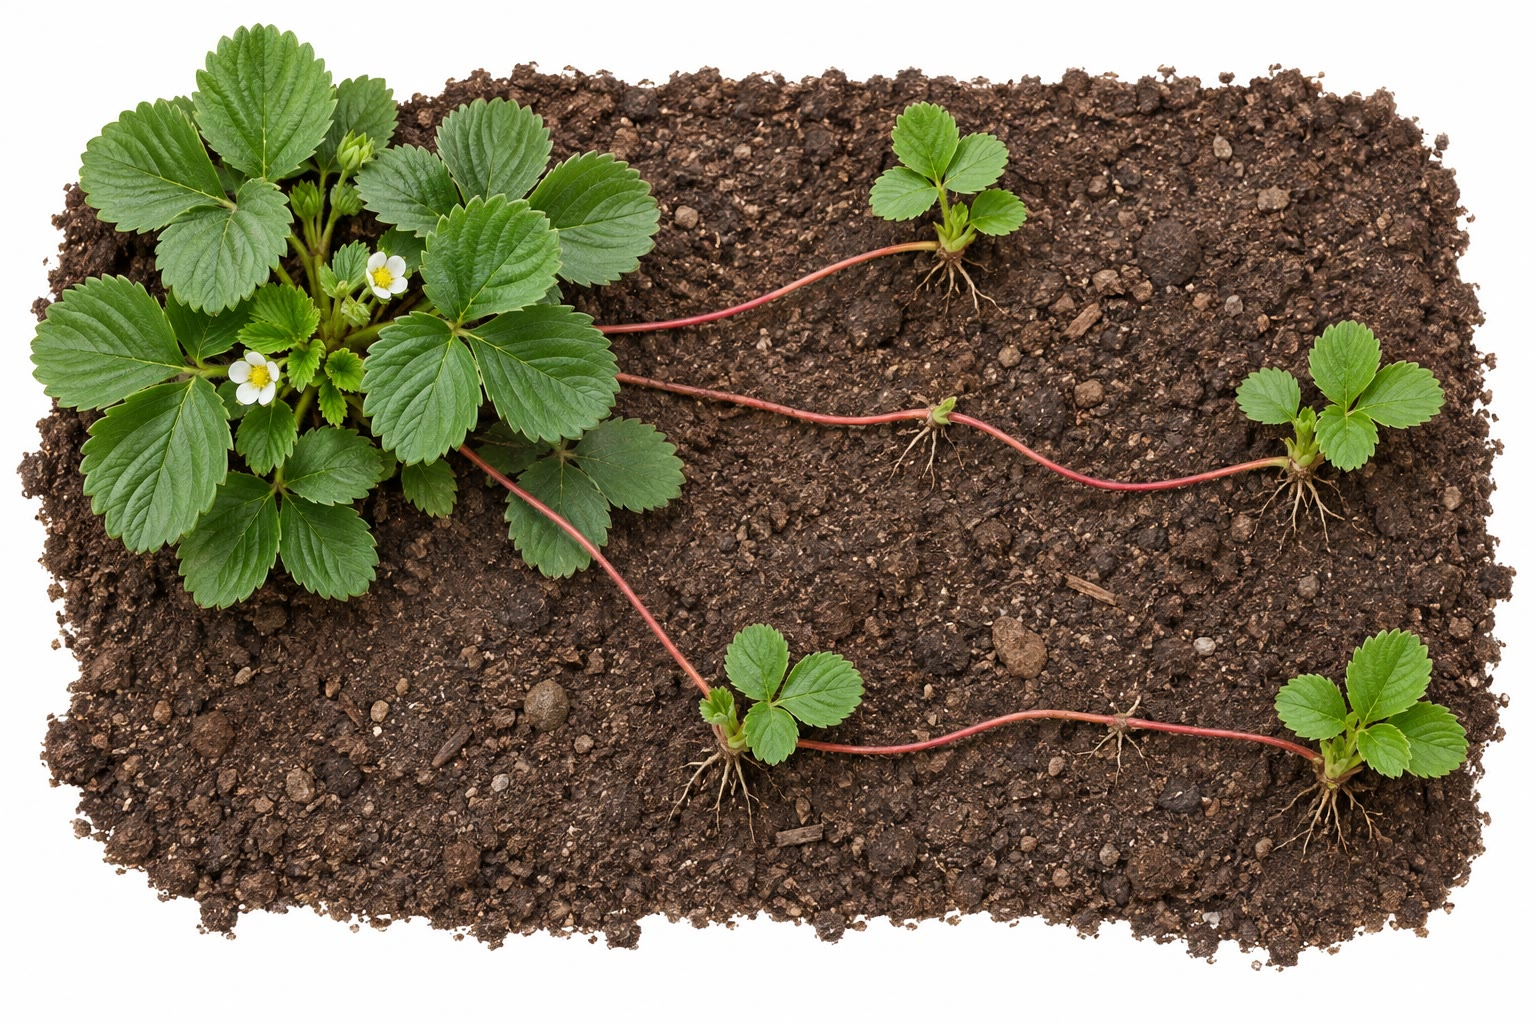
\includegraphics[width=0.46\linewidth]{images/book4/ai/b4-07-strawberry-runners.jpg}\hspace{0.03\linewidth}
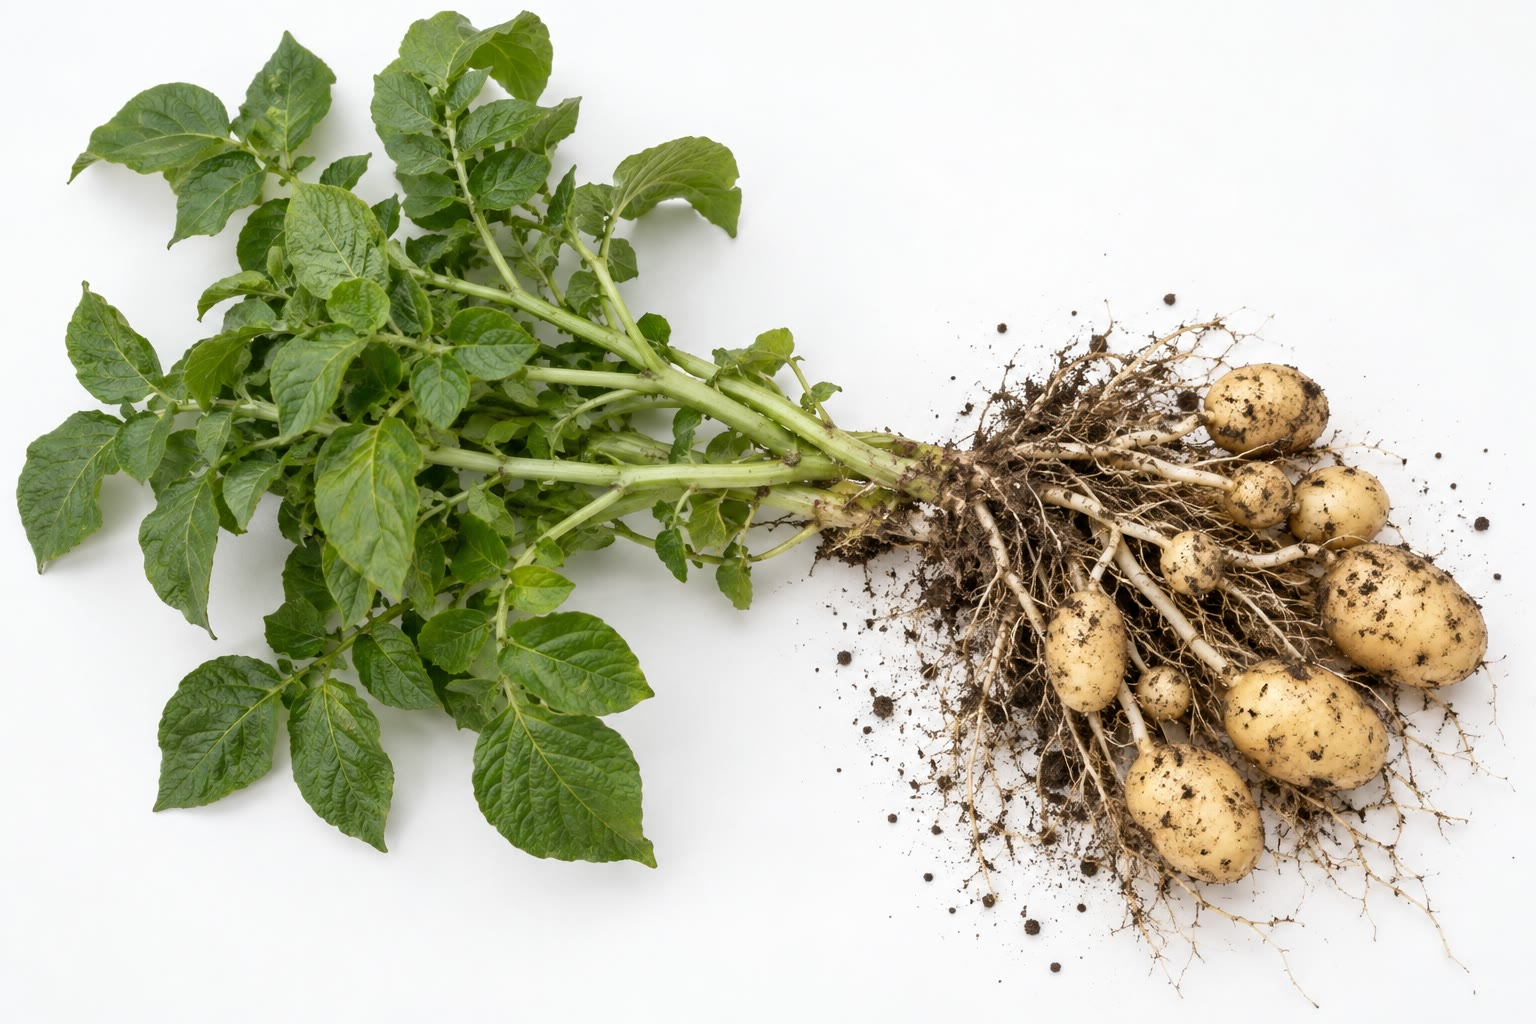
\includegraphics[width=0.46\linewidth]{images/book4/ai/b4-07-potato-tubers.jpg}

{\small Kiri: sebatang tumbuhan arbei dan tumbuhan anak yang berakar di
sepanjang sulurnya. Kanan: sebatang tumbuhan kentang yang diangkat dari
tanahnya, \omterm{prop:b2:asexual-reproduction:organs}{umbi batangnya} bergantung pada stolon --- tiap umbinya
sekeping batang yang akan tumbuh menjadi tumbuhan yang serupa secara
genetik dengan tumbuhan ini.}
\end{omfigure}

\begin{theorem}[Geometri sebuah klon yang menyebar]\label{thm:b2:asexual-reproduction:spread}
\index{pertumbuhan klonal}
Sebuah \omterm{def:b2:asexual-reproduction:clone}{genet} yang tiap \omterm{def:b2:asexual-reproduction:clone}{rametnya} menghasilkan $m$ anak berakar tiap
tahun, semuanya bertahan hidup, tumbuh cacahnya sebagai
$N(t) = N_0 (1 + m)^t$ --- pertumbuhan eksponensial tanpa seks sama
sekali --- sampai \omterm{def:b2:asexual-reproduction:clone}{rametnya} memenuhi ruangnya pada kerapatan daya
dukungnya $d$ (\omterm{def:b2:asexual-reproduction:clone}{ramet} tiap satuan luas), dan sesudah itu \omterm{def:b2:asexual-reproduction:clone}{klonnya} maju
sebagai sebuah muka. Sebuah \omterm{def:b2:asexual-reproduction:clone}{klon} yang menyebarkan sulurnya dalam garis
lurus pada kelajuan $v$ memiliki, sesudah $t$ tahun, jari-jari $vt$,
dan cacah \omterm{def:b2:asexual-reproduction:clone}{rametnya} tumbuh sebagai $\pi d (vt)^2$: secara kuadratik,
bukan eksponensial. Sebatang tumbuhan arbei yang menjulurkan sulur
\qty{0.5}{m} tiap tahun memiliki jari-jari \qty{5}{m} sesudah sepuluh
tahun; \omterm{def:b2:asexual-reproduction:clone}{klon} aspen pada alinea pembuka, seluas \qty{43}{ha}, berjari-jari
sekitar \qty{370}{m} dan, pada kemajuan neto beberapa sentimeter tiap
tahun, berumur seorde $10^{4}$ tahun --- sepadan dengan umur yang
ditaksir dari surutnya gletser.
\end{theorem}
\begin{proof}
Tiap tahunnya tiap \omterm{def:b2:asexual-reproduction:clone}{rametnya} digantikan dirinya sendiri ditambah $m$
anak, yaitu faktor $1 + m$; $t$ tahun memberi $(1 + m)^t$. Begitu
bagian dalamnya penuh, hanya \omterm{def:b2:asexual-reproduction:clone}{ramet} di tepinya yang menemukan ruang, dan
tepinya maju pada kelajuan sulurnya $v$; luasnya adalah $\pi(vt)^2$ dan
cacah \omterm{def:b2:asexual-reproduction:clone}{rametnya} adalah luasnya dikalikan kerapatannya.
\end{proof}

\begin{example}[Organisme yang tertua]\label{ex:b2:asexual-reproduction:oldest}
\omterm{def:b2:asexual-reproduction:clone}{Klon} aspen Pando (Utah) menutupi \qty{43}{ha} dengan sekitar
\num{47000} batang yang masing-masing hidup kira-kira seabad lalu
digantikan tunas akar dari akar yang sama; \omterm{def:b2:asexual-reproduction:clone}{genetnya} mungkin berumur
lebih dari sepuluh ribu tahun. Sebuah \omterm{def:b2:asexual-reproduction:clone}{klon} lamun \emph{Posidonia} di
Laut Tengah terentang \qty{15}{km} dan mungkin berumur seratus ribu
tahun; sebuah cincin semak kreosot di Mojave telah bertarikh
\num{11700} tahun, batang pusatnya mati sembari cincinnya meluas. Pada
tiap kasusnya yang tua adalah \omterm{def:b2:asexual-reproduction:clone}{genetnya}; tidak ada satu pun selnya yang
lebih tua daripada beberapa dasawarsa, dan genomnya telah disalin
ribuan kali.
\end{example}

\section{Biji tanpa seks, dan hewan tanpa ayah}

\begin{definition}[Apomiksis]\label{def:b2:asexual-reproduction:apomixis}
\index{apomiksis}\index{partenogenesis}
\emph{Apomiksis} adalah penghasilan \omterm{def:b2:angiosperm-reproduction:seed}{biji} tanpa pembuahan: sebuah
lembaga berkembang dari sel telur yang tak tereduksi (sel induk
\omterm{def:b2:plant-life-cycles:heterospory}{megasporanya} melewatkan \omterm{def:b2:meiosis-heredity:meiosis}{meiosis}) atau langsung dari sebuah sel
nuselusnya, dan \omterm{def:b2:angiosperm-reproduction:seed}{bijinya} mengusung \omterm{def:b2:meiosis-heredity:vocabulary}{genotipe} induknya. Rambutan kuning,
hawkweed, arbei hitam, rumput biru Kentucky, dan banyak jeruk
melakukannya; \omterm{def:b2:angiosperm-reproduction:seed}{biji} jeruk kerap memuat beberapa lembaga, satu seksual
dan sisanya salinan nuselus induknya. Apomiksis mempertahankan \omterm{def:b2:angiosperm-reproduction:seed}{bijinya}
--- penyebarannya, \omterm{def:b2:angiosperm-reproduction:seed}{dormansinya}, dan kulitnya --- lalu melepaskan
\omterm{def:b2:meiosis-heredity:meiosis}{meiosisnya}, sehingga \omterm{def:b2:meiosis-heredity:vocabulary}{genotipe} yang teradaptasi baik disiarkan tanpa
berubah; sebagian besar apomik adalah \omterm{def:b2:genome-diversification:polyploidy}{poliploid} berasal hibrid yang
\omterm{def:b2:meiosis-heredity:meiosis}{meiosisnya} toh akan gagal. Padanannya pada hewan adalah
\emph{partenogenesis}, yaitu perkembangan dari telur yang tak dibuahi:
wajib pada sebagian kadal dan pada rotifera bdeloid, yang tidak
memiliki jantan selama puluhan juta tahun; berdaur pada kutu daun dan
kutu air, yang berbiak secara partenogenetik sepanjang musim panas,
seekor betina melahirkan anak betina hidup yang sudah mengusung
lembaganya sendiri, lalu beralih ke sebuah generasi seksual pada musim
gugur yang bertelur untuk melewati musim dingin.
\end{definition}

\begin{omfigure}
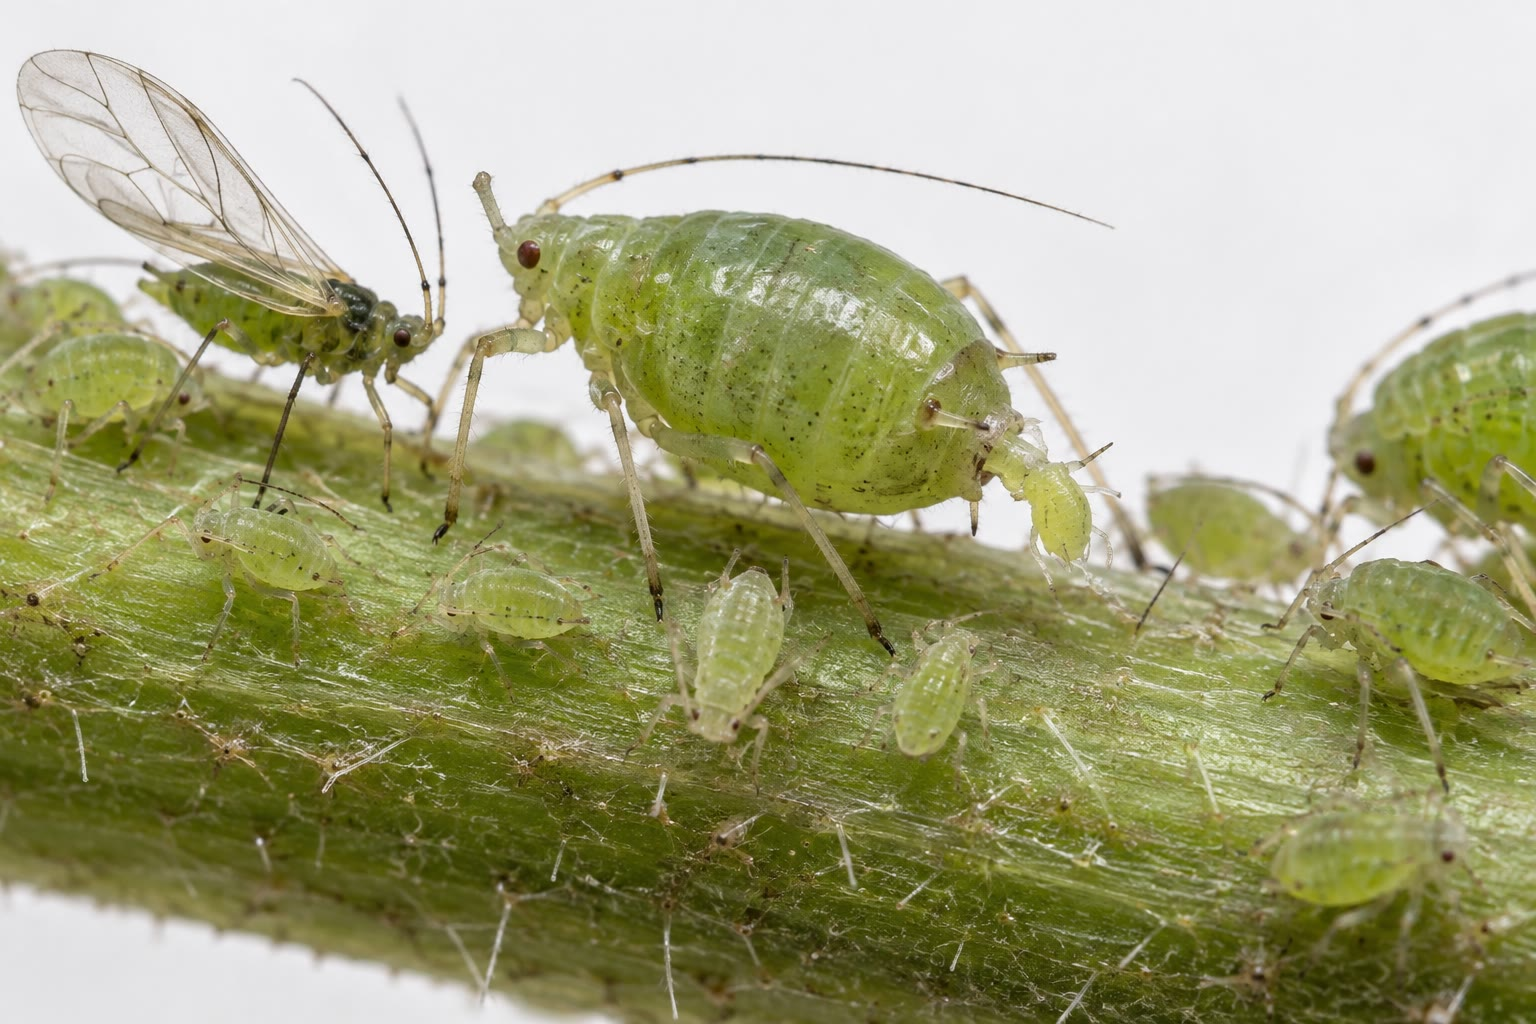
\includegraphics[width=0.55\linewidth]{images/book4/ai/b4-07-aphids.jpg}

{\small Kutu daun pada sebatang batang: seekor betina partenogenetik
tanpa sayap yang melahirkan seekor anak betina hidup, nimfa dari
beberapa umur, dan seekor pendatang bersayap --- pertumbuhan
eksponensial satu musim panas tanpa seekor jantan pun.}
\end{omfigure}

\begin{example}[Satu musim panas kutu daun]\label{ex:b2:asexual-reproduction:aphids}
Seekor kutu daun partenogenetik matang dalam kira-kira delapan hari
lalu menghasilkan sekitar lima anak betina tiap hari selama dua pekan;
anaknya lahir sudah hamil (lembaganya mulai berkembang di dalam lembaga
induknya). Dengan \omterm{def:b2:unicellular-diversity:division}{waktu generasi} mendekati sepuluh hari dan laju
kenaikan neto sekitar \num{50} tiap generasi, satu pendiri pada bulan
April dapat, tanpa terkendali, meninggalkan
$50^{12} \approx 2\times 10^{20}$ keturunan dalam empat bulan --- lebih
besar massanya daripada
tiap hewan yang kini hidup. Kumbang koksi, undur-undur, tawon
parasitoid, fungi, dan hujan menahan cacahnya sampai beberapa ribu tiap
tumbuhannya, dan generasi seksual musim gugurnya menyetel ulang \omterm{def:b2:asexual-reproduction:clone}{klonnya}
menjadi telur hasil rekombinasi sebelum musim dingin.
\end{example}

\section{Pengklonaan oleh pekebun}

\begin{proposition}[Setek, pencangkokan, penyambungan]\label{prop:b2:asexual-reproduction:horticulture}
\index{setek}\index{penyambungan}\index{batang bawah}
Sebuah \emph{setek} adalah sekeping batang, akar, atau daun yang
diimbas berakar: ujung potongannya membentuk kalus berisi sel yang
membelah, dan darinya meristem akar muncul, dibantu auksin (hormon
pengakaran) serta kelembapan. \emph{Pencangkokan} mengakarkan sebuah
cabang selagi masih melekat lalu memotongnya sesudahnya.
\emph{Penyambungan} menggabungkan pucuk satu tumbuhan (\emph{batang
atas}) dengan batang berakar tumbuhan lain (\emph{\omterm{prop:b2:asexual-reproduction:horticulture}{batang bawah}}):
kedua kambiumnya ditekankan bersama, kalusnya menjembatani lukanya, dan
xilem serta floem yang baru tersambung menyeberanginya dalam beberapa
pekan. Sambungannya adalah sebuah kimera --- akarnya mempertahankan
genom \omterm{prop:b2:asexual-reproduction:horticulture}{batang bawahnya}, pucuk berbuahnya genom batang atasnya --- dan ia
hanya berhasil antara tumbuhan yang berkerabat (spesies satu marga,
kadang satu suku), karena jaringannya harus mengenali sel satu sama
lain. Tiap varietas apel, pir, ceri, jeruk, dan anggur diperbanyak
lewat penyambungan: sebuah varietas bernama adalah satu \omterm{def:b2:asexual-reproduction:clone}{genet}, yang
dijaga hidup berabad-abad lewat batang atas (apel Reinette bertarikh
dari abad keenam belas), dan \omterm{prop:b2:asexual-reproduction:horticulture}{batang bawahnya} dipilih menurut tanahnya,
penyakitnya, dan ukuran pohon yang diinginkan --- \omterm{prop:b2:asexual-reproduction:horticulture}{batang bawah} pengerdil
menghasilkan pohon kecil kebun modern.
\end{proposition}

\begin{proposition}[Mikropropagasi dan ketotipotenan]\label{prop:b2:asexual-reproduction:tissueculture}
\index{mikropropagasi}\index{ketotipotenan}\index{kalus}
Tiap sel tumbuhan yang hidup dan berinti dapat, pada asasnya,
meregenerasikan seluruh tumbuhan. Dalam \emph{kultur jaringan}
sekeping jaringan yang disterilkan (sebuah \emph{eksplan}: ujung
pucuk, cakram daun, kepala sari) diletakkan pada medium agar dengan
gula, mineral, vitamin, dan hormon. Dengan auksin dan sitokinin yang
seimbang, selnya bernyahdiferensiasi menjadi sebuah \emph{kalus}, yaitu
massa sel tak terkhusus yang membelah; dengan sitokinin lebih banyak
daripada auksin, kalusnya membentuk pucuk, dengan auksin lebih banyak
daripada sitokinin ia membentuk akar, dan pada sebagian spesies ia
membentuk \emph{lembaga soma} --- lembaga lengkap tanpa sebuah sel
telur. Pucuknya dipotong lalu disubkultur tiap beberapa pekan, dan
berlipat ganda dengan faktor tiga sampai sepuluh tiap kalinya, sehingga
satu meristem memberi sejuta tumbuhan kecil dalam setahun. Karena
virusnya tertinggal di belakang ujung yang tumbuh, sebuah meristem
pucuk yang panjangnya kurang dari satu milimeter biasanya bebas virus
bahkan pada tumbuhan yang terjangkiti: \emph{kultur meristem} adalah
cara stok kentang, arbei, pisang, dan anggrek dibersihkan. Metodenya
adalah bukti praktis ketotipotenan, dan alasan sebuah varietas tumbuhan
dapat dijual berjuta-juta dalam beberapa tahun sesudah penciptaannya.
\end{proposition}
\begin{proof}[Bukti eksperimental]
Skoog dan Miller (1957) menumbuhkan kalus empulur tembakau pada medium
dengan rasio auksin terhadap sitokinin yang baru ditemukan yang
berbeda-beda: auksin tinggi memberi akar, sitokinin tinggi memberi
pucuk, keseimbangannya hanya memberi kalus --- pembentukan organnya
ditetapkan sebuah rasio dua hormon, bukan sebuah zat khusus pembentuk
organ. Steward (1958) menggantung sel tunggal dan gumpalan kecil dari
sebuah akar wortel di dalam labu berputar berisi air kelapa: sebagian
gumpalannya membentuk struktur mirip lembaga yang tumbuh menjadi wortel
utuh yang berbunga, yang menunjukkan bahwa sebuah sel yang
terdiferensiasi dari organ yang matang masih memuat, dan dapat memakai,
seluruh program perkembangannya.
\end{proof}

\begin{omfigure}
\begin{tikzpicture}[every node/.style={font=\scriptsize}, >=stealth]
  \node[draw, rounded corners, fill=omDef!12, align=center] (ex) at (0,0) {eksplan\\(ujung pucuk, cakram daun)};
  \node[draw, rounded corners, fill=omExo!30, align=center] (cal) at (4.6,0) {kalus\\auksin $\approx$ sitokinin};
  \node[draw, rounded corners, fill=omExo!30, align=center] (sh) at (8.4,1.2) {pucuk\\sitokinin $>$ auksin};
  \node[draw, rounded corners, fill=omExo!30, align=center] (rt) at (8.4,-1.2) {akar\\auksin $>$ sitokinin};
  \node[draw, rounded corners, fill=omDef!12, align=center] (pl) at (12.2,0) {tumbuhan kecil\\diaklimatisasi di tanah};
  \draw[->, thick] (ex) -- (cal) node[midway, below, align=center] {medium\\steril};
  \draw[->, thick] (cal) -- (sh); \draw[->, thick] (cal) -- (rt);
  \draw[->, thick] (sh) -- (pl); \draw[->, thick] (rt) -- (pl);
  \draw[->, thick, omThm] (sh) .. controls (8.4,2.6) and (5.8,2.6) .. (5.2,0.6);
  \node[omThm, anchor=south] at (6.9,2.3) {subkultur tiap 4 pekan, $\times 5$};
\end{tikzpicture}

{\small Mikropropagasi: sebuah eksplan dinyahdiferensiasikan menjadi
sebuah kalus, diarahkan menjadi pucuk atau akar oleh rasio auksin
terhadap sitokinin, lalu dilipatgandakan lewat subkultur berulang
sebelum tumbuhan kecilnya disapih ke tanah.}
\end{omfigure}

\begin{omfigure}
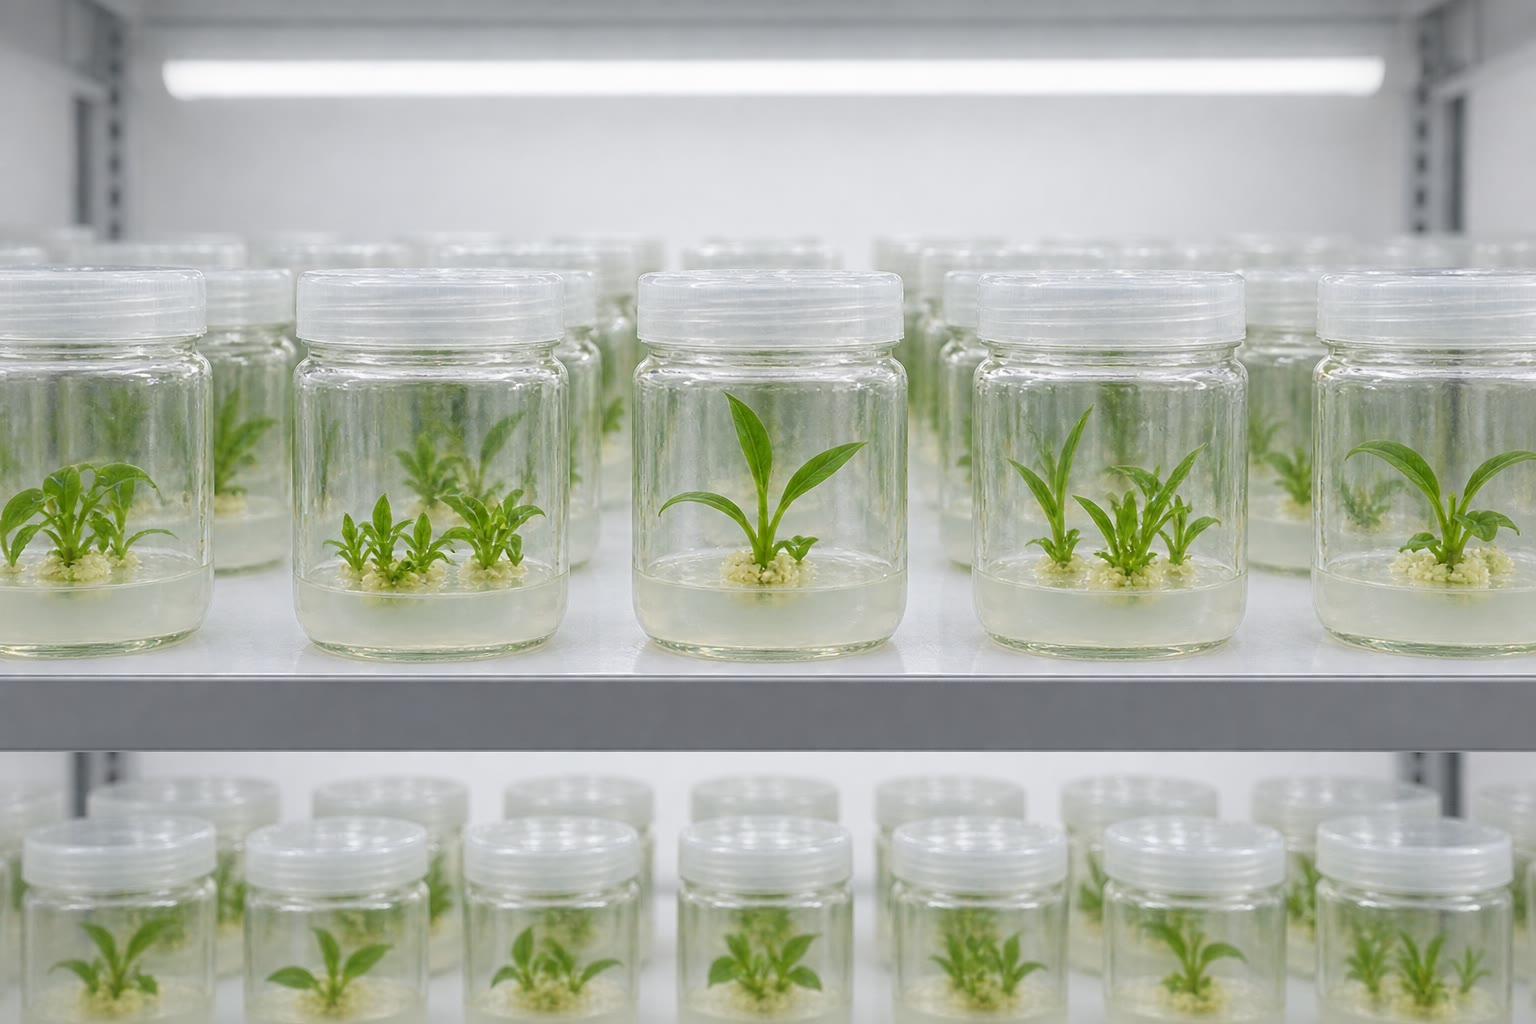
\includegraphics[width=0.6\linewidth]{images/book4/ai/b4-07-tissue-culture.jpg}

{\small Tumbuhan kecil di atas agar di dalam ruang tumbuh: tiap
toplesnya memuat sebuah \omterm{def:b2:asexual-reproduction:clone}{klon} varietas yang sama, dilipatgandakan dari
satu meristem.}
\end{omfigure}

\section{Ongkos seks dan ongkos tanpa seks}

\begin{theorem}[Ongkos dua kali lipat seks]\label{thm:b2:asexual-reproduction:twofold}
\index{ongkos dua kali lipat seks}
Pada populasi yang tiap betinanya membuat $F$ keturunan, separuhnya
anak jantan, seekor betina mutan aseksual yang membuat $F$ anak betina,
semuanya salinan dirinya sendiri, melipatduakan bagiannya atas betina
generasi berikutnya. Kalau garis keturunan aseksualnya berfrekuensi $p$
di antara betinanya, maka pada generasi berikutnya
\[
p' = \frac{2p}{1 + p}, \qquad p_t = \frac{2^t p_0}{1 + (2^t - 1)p_0},
\]
sehingga dari satu per seribu ia mencapai separuh populasinya dalam
sepuluh generasi dan seluruhnya tak lama sesudah itu. Dengan segala
hal lain setara, seks memerohkan laju pelipatgandaan sebuah garis
keturunan --- itulah harga membuat jantan. Karena seks toh nyaris
mendunia, segala hal lain memang tidak setara: garis keturunan seksual
haruslah, secara rata-rata, memperoleh sedikitnya faktor dua dari
rekombinasinya.
\end{theorem}
\begin{proof}
Betina aseksualnya berjumlah $pN$ dan meninggalkan $FpN$ anak betina;
betina seksualnya berjumlah $(1 - p)N$ dan meninggalkan $F(1 - p)N/2$
anak betina (separuhnya yang lain adalah anak jantan, yang tidak
membuat telur). Bagian aseksual atas anak betinanya adalah
$Fp/(Fp + F(1 - p)/2) = 2p/(1 + p)$. Dengan menuliskan $q = p/(1 -
p)$, rekursinya menjadi $q' = 2q$, sehingga $q_t = 2^t q_0$; mengubahnya
kembali memberi $p_t$. Menetapkan $p_t = \tfrac12$ memberi $2^t q_0 = 1$, yakni
$t = \log_2(1/q_0) \approx 10$ bagi $p_0 = 10^{-3}$.
\end{proof}

\begin{omfigure}
\begin{tikzpicture}
\begin{axis}[
  width=0.76\linewidth, height=5.6cm,
  axis x line=bottom, axis y line=left,
  xmin=0, xmax=20, ymin=0, ymax=1.05,
  xlabel={generasi}, ylabel={frekuensi garis keturunan aseksualnya},
  xlabel style={font=\small, at={(axis description cs:0.5,-0.13)}, anchor=north},
  ylabel style={font=\small},
  tick label style={font=\small}, xtick={0,5,10,15,20}, ytick={0,0.5,1},
  legend style={font=\scriptsize, at={(0.5,-0.3)}, anchor=north, draw=none},
  clip=false,
]
\addplot[very thick, omThm, domain=0:20, samples=80] {2^x*0.001/(1+(2^x-1)*0.001)};
\addlegendentry{tanpa perbedaan lain: mengambil alih dalam 12 generasi}
\addplot[very thick, omDef, domain=0:20, samples=80] {0.001*(1.3)^x/(1+(1.3^x-1)*0.001)};
\addlegendentry{kaum aseksual kehilangan \qty{35}{\%} kebugaran karena parasit: lebih lambat}
\addplot[very thick, omProp, domain=0:20, samples=80] {0.001*(0.9)^x/(1+(0.9^x-1)*0.001)};
\addlegendentry{kaum aseksual kehilangan \qty{55}{\%}: mereka tak pernah menyebar}
\end{axis}
\end{tikzpicture}

{\small Keunggulan dua kali lipat itu dalam tindakan. Dimulai pada satu
per seribu, sebuah garis keturunan aseksual tanpa kerugian lain
mengambil alih dalam selusin generasi; hanya denda kebugaran sedikitnya
separuh --- dari parasit, \omterm{def:b2:genome-diversification:mutation}{mutasi} yang menimbun, atau adaptasi yang
lebih lambat --- yang menahannya.}
\end{omfigure}

\begin{proposition}[Untuk apa seks]\label{prop:b2:asexual-reproduction:whysex}
\index{ratchet Muller}\index{hipotesis Ratu Merah}
Ada tiga manfaat yang cukup besar untuk berarti. \emph{\omterm{prop:b2:asexual-reproduction:whysex}{Ratchet
Muller}}: di dalam sebuah \omterm{def:b2:asexual-reproduction:clone}{klon}, tiap \omterm{def:b2:genome-diversification:mutation}{mutasi} yang merugikan diwarisi
seluruh keturunannya, dan sebuah genom bebas \omterm{def:b2:genome-diversification:mutation}{mutasi}, begitu hilang dari
populasi berhingga secara kebetulan, tidak pernah dapat dibuat kembali;
bebannya bergerigi naik, satu ketukan demi satu ketukan, dan populasi
aseksual yang kecil meluruh. Rekombinasi membangun kembali genom yang
bersih dari dua genom yang rusak. \emph{Adaptasi}: dua \omterm{def:b2:genome-diversification:mutation}{mutasi} yang
berguna yang muncul pada individu berbeda sebuah \omterm{def:b2:asexual-reproduction:clone}{klon} bersaing dan
salah satunya hilang; pada populasi seksual keduanya bergabung (Fisher
dan Muller, 1930-an), sehingga populasi seksual beradaptasi lebih cepat
ketika banyak gen harus berubah. \emph{Ratu Merah}: parasit
beradaptasi kepada \omterm{def:b2:meiosis-heredity:vocabulary}{genotipe} inang yang paling lazim, dan sebuah \omterm{def:b2:asexual-reproduction:clone}{klon},
karena ia satu \omterm{def:b2:meiosis-heredity:vocabulary}{genotipe}, adalah yang paling lazim dari semuanya; tetua
seksual menjadikan tiap keturunannya sebuah gembok baru. Siput, ikan,
dan tumbuhan yang memiliki populasi seksual sekaligus klonal
menunjukkan populasi seksualnya yang menang di tempat parasitnya
berlimpah. Garis keturunan aseksual yang berkembang --- rambutan
kuning, rotifera bdeloid, sebagian besar \omterm{def:b2:asexual-reproduction:clone}{klon} tanaman budi daya ---
entah masih muda, atau merupakan hibrid \omterm{def:b2:genome-diversification:polyploidy}{poliploid} yang mengusung
keragamannya sendiri, atau ditopang seorang pekebun yang membunuh
parasitnya untuk mereka.
\end{proposition}

\begin{example}[Monokultur sebuah klon]\label{ex:b2:asexual-reproduction:monoculture}
Pada 1840-an sebagian besar panen kentang Irlandia adalah satu varietas
klonal, yaitu Lumper; kapang air \emph{Phytophthora infestans}, yang
tiba pada 1845, berjumpa dengan sebuah negeri berisi tumbuhan yang
serupa secara genetik dan seragam kepekaannya lalu memusnahkan
panennya tiga tahun berturut-turut. Pisang ekspor dunia sampai 1950-an
adalah satu \omterm{def:b2:asexual-reproduction:clone}{klon} tunggal, yaitu Gros Michel, yang dilenyapkan dari
perkebunan Amerika Tengah oleh sejenis fungi tanah; penggantinya,
Cavendish, juga satu \omterm{def:b2:asexual-reproduction:clone}{klon} tunggal dan kini sedang hilang, perkebunan
demi perkebunan, oleh galur baru fungi yang sama, dan terhadapnya ia
tidak punya keragaman apa pun untuk ditawarkan. Sebuah \omterm{def:b2:asexual-reproduction:clone}{klon} adalah
sasaran termudah di alam, dan pekebun yang menanam satu \omterm{def:b2:asexual-reproduction:clone}{klon} harus
memasok kekebalan yang akan dipasok rekombinasi secara cuma-cuma.
\end{example}

\section{Latihan}

\begin{exercise}[$\star$]\label{exo:b2:asexual-reproduction:1}
Definisikan \omterm{def:b2:asexual-reproduction:clone}{klon}, \omterm{def:b2:asexual-reproduction:clone}{genet}, dan \omterm{def:b2:asexual-reproduction:clone}{ramet}, lalu berikan tiga organ alami
\omterm{def:b2:asexual-reproduction:clone}{pelipatgandaan vegetatif} beserta sebuah tumbuhan bagi masing-masing.
\end{exercise}

\begin{exercise}[$\star$]\label{exo:b2:asexual-reproduction:2}
Pada sebuah sambungan, jaringan apa yang harus bertemu agar
penyatuannya berhasil, dan apa yang disumbangkan tiap pasangannya
kepada pohonnya? Mengapa pohon sambungan adalah kimera dan bukan hibrid?
\end{exercise}

\begin{exercise}[$\star$]\label{exo:b2:asexual-reproduction:3}
Bedakanlah \omterm{def:b2:asexual-reproduction:apomixis}{apomiksis} dari \omterm{def:b2:asexual-reproduction:clone}{pelipatgandaan vegetatif}, dan
\omterm{def:b2:asexual-reproduction:apomixis}{partenogenesis} dari keduanya. Mana di antara ketiganya yang
mempertahankan \omterm{def:b2:angiosperm-reproduction:seed}{bijinya}?
\end{exercise}

\begin{exercise}[$\star$]\label{exo:b2:asexual-reproduction:4}
Daftarkan langkah mikropropagasi dari eksplan sampai tumbuhan di
ladang, sambil menamai keadaan hormonnya pada tiap langkahnya.
\end{exercise}

\begin{exercise}[$\star\star$]\label{exo:b2:asexual-reproduction:5}
Sebatang tumbuhan arbei membuat 8 sulur tiap tahun, masing-masing
mengakarkan 3 tumbuhan kecil, dan tiap tumbuhan kecilnya melakukan hal
yang sama pada tahun berikutnya. Berapa tumbuhan sesudah 4 tahun kalau
tak satu pun mati? Pada \qty{0.1}{m^2} tiap tumbuhannya, berapa luas
yang dibutuhkannya? Apa yang sesungguhnya membatasi \omterm{def:b2:asexual-reproduction:clone}{klonnya}?
\end{exercise}

\begin{exercise}[$\star\star$]\label{exo:b2:asexual-reproduction:6}
\omterm{def:b2:asexual-reproduction:clone}{Klon} aspen Pando memiliki \num{47000} batang pada \qty{43}{ha}, tiap
batangnya hidup kira-kira \num{130} tahun. Kalau \omterm{def:b2:asexual-reproduction:clone}{genetnya} berumur
\num{14000} tahun, sudah berapa generasi batang yang dimilikinya?
Hitunglah purata kemajuan jejarinya dalam meter tiap tahun, dengan
memperlakukannya sebagai sebuah cakram.
\end{exercise}

\begin{exercise}[$\star\star$]\label{exo:b2:asexual-reproduction:7}
Seorang mutan aseksual muncul pada frekuensi $10^{-4}$ di dalam sebuah
populasi seksual, dengan kesuburan yang sama. Hitunglah frekuensinya
sesudah 5, 10, dan 15 generasi. Seberapa besar kebugarannya harus
diturunkan agar ia tidak pernah menyebar?
\end{exercise}

\begin{exercise}[$\star\star$]\label{exo:b2:asexual-reproduction:8}
Ramalkanlah apa yang dikerjakan sebuah kalus tembakau pada medium
dengan rasio auksin : sitokinin 10 : 1, 1 : 1, dan 1 : 10, lalu
jelaskan mengapa setek pucuk dicelupkan ke dalam auksin, bukan
sitokinin.
\end{exercise}

\begin{exercise}[$\star\star$]\label{exo:b2:asexual-reproduction:9}
Kentang ditanam sebagai \omterm{prop:b2:asexual-reproduction:organs}{umbi batang}. Satu kilogram yang ditanam
menghasilkan \qty{10}{kg}, dan satu hektar membutuhkan \qty{2}{t} umbi
bibit. Dimulai dari \qty{1}{kg} sebuah varietas baru, berapa musim
sampai satu hektar dapat ditanami? Mengapa \omterm{def:b2:angiosperm-reproduction:seed}{biji} sejati memberi
pelipatgandaan yang lebih cepat tetapi tidak dipakai?
\end{exercise}

\begin{exercise}[$\star\star\star$]\label{exo:b2:asexual-reproduction:10}
Pada sebuah populasi klonal berisi $N$ individu dengan $U$ \omterm{def:b2:genome-diversification:mutation}{mutasi}
merugikan tiap genom tiap generasi, yang masing-masing memakan bagian
$s$ dari kebugarannya, bagian individu yang bebas \omterm{def:b2:genome-diversification:mutation}{mutasi} pada
kesetimbangannya adalah $e^{-U/s}$ (diturunkan dalam
\cref{ch:b2:population-genetics}). Dengan $U =
0.1$ dan $s = 0.02$, hitunglah cacah individu yang bebas \omterm{def:b2:genome-diversification:mutation}{mutasi} bagi
$N = 10^{5}$ dan $N = 10^{3}$, lalu jelaskan, dengan \omterm{prop:b2:asexual-reproduction:whysex}{ratchet Muller},
mengapa populasi yang kecil ditakdirkan musnah dan yang besar belum.
\end{exercise}

\begin{exercise}[$\star\star\star$]\label{exo:b2:asexual-reproduction:11}
Sebuah galur patogen yang mengalahkan kekebalan sebuah \omterm{def:b2:meiosis-heredity:vocabulary}{genotipe}
tertentu muncul satu kali. Bandingkanlah nasibnya di dalam sebuah ladang
berisi satu \omterm{def:b2:asexual-reproduction:clone}{klon} dan di dalam sebuah populasi seksual yang gen
kekebalannya memilah pada sepuluh lokus, masing-masing dengan dua \omterm{def:b2:meiosis-heredity:vocabulary}{alel}
yang sama frekuensinya, lalu jelaskan bencana kelaparan kentang
Irlandia dari segi itu.
\end{exercise}

\begin{exercise}[$\star\star\star$]\label{exo:b2:asexual-reproduction:12}
``Seks berongkos faktor dua dan ada di mana-mana; keaseksualan murah
dan langka.'' Bahaslah ketiga penjelasan bab ini, lalu katakan apa yang
disiratkan rotifera bdeloid --- yang aseksual selama empat puluh juta
tahun --- bagi masing-masingnya.
\end{exercise}

\section{Soal: Sebuah Kebun Arbei dan Sebuah Klon Tua}

\begin{problem}[{Soal akhir pekan --- aritmetika sebuah klon, dari
sebuah ladang arbei yang dipenuhi sulur dan sebuah laboratorium yang
melipatgandakan sebuah meristem, sampai ke penyerbuan sebuah populasi
seksual oleh seorang apomik dan pembusukan genetik sebuah genet purba,
berakhir pada waktu memenuhi ladangnya, tumbuhan kecil dari satu
meristem, dan kesetimbangan kaum apomik dan kaum seksual}]
\label{pb:b2:asexual-reproduction:1}
Seorang pekebun menanam \num{100} tumbuhan arbei di sebuah ladang
seluas \qty{1}{ha} yang sanggup mendukung \num{4} tumbuhan tiap meter
persegi. Tiap tumbuhannya membuat \num{6} sulur tiap tahun,
masing-masing mengakarkan \num{2} anak, dan semua tumbuhannya bertahan
hidup. Sebuah laboratorium melipatgandakan varietas yang sama lewat
kultur jaringan: tiap subkultur, tiap \num{4} pekan, melipatgandakan
pucuknya dengan \num{5}; \qty{80}{\%} tumbuhan kecilnya selamat dari
penyapihan. Setek biasa varietas itu \qty{90}{\%} terjangkiti virus;
ujung meristem \qty{0.3}{mm} mengusung virusnya dengan peluang
$0.02$. Genom aspennya: \qty{4.8e8}{} pasangan basa; \omterm{thm:b2:genome-diversification:rate}{laju mutasi}
somanya \qty{1e-9}{} tiap pasangan basa tiap pembelahan sel; \num{20}
pembelahan sel meristem tiap tahun pada pucuk yang tumbuh.

\medskip
\noindent\textbf{Bagian I --- Memenuhi ladangnya.}
\begin{enumerate}
  \item Berapa tumbuhan yang dapat ditampung ladangnya?
  \item Dengan faktor berapa cacah tumbuhannya berlipat ganda tiap
        tahun?
  \item Hitunglah cacah tumbuhannya sesudah 1, 2, dan 3 tahun.
  \item Pecahkanlah $N(t) = 100\times 13^{t}$ untuk waktu saat
        ladangnya penuh.
  \item Begitu penuh, hanya tumbuhan di tepi sebuah petak yang
        menemukan ruang. Kalau sebuah petak maju \qty{0.5}{m} tiap
        tahun, berapa tahun yang dibutuhkan satu tumbuhan untuk
        menutupi ladangnya lewat kemajuan semata?
  \item Jelaskan mengapa pekebunnya menanam \num{100} tumbuhan yang
        tersebar di ladangnya alih-alih satu tumbuhan.
\end{enumerate}

\medskip
\noindent\textbf{Bagian II --- Laboratoriumnya.}
\begin{enumerate}[resume]
  \item Berapa subkultur yang dibutuhkan untuk beranjak dari satu
        meristem ke sedikitnya $10^{6}$ pucuk? Berapa pekan?
  \item Berapa tumbuhan yang selamat dari penyapihan?
  \item Berapa peluang bahwa sebuah galur asal meristem bebas virus?
        Bahwa \num{10} galur yang dimulai dari satu tumbuhan semuanya
        bebas virus?
  \item Laboratoriumnya memulai \num{10} galur lalu membuang yang
        terjangkiti sesudah sebuah uji. Berapa harapan cacah galur yang
        bersih? Bandingkan dengan seteknya.
  \item Jelaskan mengapa ujung meristemnya lolos dari virusnya.
  \item Ladangnya dapat ditanami dari keluaran laboratoriumnya pada
        tahun pertama alih-alih dipenuhi sulur dalam tiga tahun.
        Berikan satu keunggulan dan satu risiko tiap jalannya.
\end{enumerate}

\medskip
\noindent\textbf{Bagian III --- Seorang apomik menyerbu.}
Sebuah populasi rambutan kuning bersifat seksual; seorang mutan apomik
(pengklon lewat \omterm{def:b2:angiosperm-reproduction:seed}{biji}) muncul pada frekuensi $p_0 = 10^{-3}$ dengan
keluaran \omterm{def:b2:angiosperm-reproduction:seed}{biji} tiap tumbuhan yang sama. Separuh upaya perkembangbiakan
tumbuhan seksualnya masuk ke \omterm{def:b2:plant-life-cycles:heterospory}{serbuk sari}.
\begin{enumerate}[resume]
  \item Berilah alasan bagi rekursi $p' = 2p/(1 + p)$ bagi frekuensi
        apomiknya di antara tetua \omterm{def:b2:angiosperm-reproduction:seed}{bijinya}.
  \item Hitunglah $p$ sesudah 5 dan 10 generasi, serta generasi saat ia
        melewati separuh.
  \item Sejenis fungi karat mengkhusus pada \omterm{def:b2:meiosis-heredity:vocabulary}{genotipe} yang paling lazim:
        keluaran \omterm{def:b2:angiosperm-reproduction:seed}{biji} apomiknya turun dengan faktor $(1 - cp)$, dengan
        $c = 0.8$. Tuliskanlah rekursi yang baru.
  \item Carilah frekuensi kesetimbangannya $p^*$ lalu periksalah
        kemantapannya dari tanda $p' - p$ pada kedua sisinya.
  \item Bagi nilai $c$ yang mana apomiknya mengambil alih seluruhnya?
  \item Hitunglah kesetimbangannya bagi $c = 0.6$. Tafsirkanlah: apa
        yang harus dikerjakan sebuah parasit untuk melindungi seks?
  \item Apomiknya adalah sebuah triploid. Mengapa ia tidak dapat
        kembali kepada seks, dan mengapa hal itu berarti dalam jangka
        panjang?
\end{enumerate}

\medskip
\noindent\textbf{Bagian IV --- \omterm{def:b2:asexual-reproduction:clone}{Klon} tuanya.}
\begin{enumerate}[resume]
  \item Hitunglah cacah \omterm{def:b2:genome-diversification:mutation}{mutasi} soma tiap pembelahan sel pada aspennya.
  \item Dua batang \omterm{def:b2:asexual-reproduction:clone}{klon} Pando dipisahkan \num{14000} tahun pertumbuhan
        pada tiap sisi moyang bersamanya. Berapa pembelahan sel yang
        memisahkan keduanya, dan berapa \omterm{def:b2:genome-diversification:mutation}{mutasi} yang membedakan
        genomnya?
  \item Berapa bagian genomnya itu? Kalau \qty{2}{\%} genomnya
        menyandi, berapa perbedaan penyandinya?
  \item Sebuah \omterm{def:b2:asexual-reproduction:clone}{klon} tidak memiliki \omterm{def:b2:meiosis-heredity:meiosis}{meiosis} dan tidak memiliki seleksi
        pada taraf organisme untuk membuang \omterm{def:b2:genome-diversification:mutation}{mutasi} ini. Apa yang
        membuangnya, dan mengapa ayakannya lebih lemah daripada pada
        garis keturunan seksual?
  \item Apakah Pando ``seragam secara genetik''? Bahaslah dalam dua
        kalimat.
  \item Nyatakan hasilnya: waktu memenuhi ladangnya lewat sulur,
        tumbuhan kecil yang diberikan satu meristem dalam setahun, dan
        frekuensi kesetimbangan apomiknya bagi $c = 0.8$.
\end{enumerate}
\end{problem}
